\documentclass[10pt]{beamer}

\usepackage[utf8]{inputenc}
\usepackage[spanish]{babel}
\usepackage{graphicx}

\mode<presentation>
\usetheme{Madrid}
%\usecolortheme[RGB={111,73,135}]{structure}
\usecolortheme[RGB={128,0,0}]{structure}
%\usecolortheme[RGB={0,96,0}]{structure}
%\usecolortheme[RGB={200,0,200}]{structure}
%\usecolortheme[RGB={0,128,0}]{structure}
%\usecolortheme[RGB={0,0,128}]{structure}
\usefonttheme{serif}
\useinnertheme{rectangles}
\useoutertheme{split}

\setbeamercovered{transparent}

\title{Desarrollo de aplicaciones Python-GTK}
\author{Jesús Espino García}
\date{15 de Julio de 2011}
\subject{Desarrollo de aplicaciones Python-GTK}

\institute[Python Madrid 2011]{Kaleidos\\Python Madrid 2011}

\setcounter{tocdepth}{2}

\AtBeginSubsection[]
{
  \begin{frame}<beamer>{Indice}
    \tableofcontents[sectionstyle=show/shaded,subsectionstyle=show/shaded/hide]
  \end{frame}
}

\begin{document}

  \frame{\maketitle}

  \section{Introducción}
  \begin{frame}[containsverbatim]
    \frametitle{¿Por qué PyGTK?}

    \begin{itemize}
      \item Es Python!!
      \item Es totalmente libre (Python y GTK).
      \item Es rápido de aprender.
      \item Es rápido de desarrollar.
      \item Bien documentado.
      \item Lo aprendido sirve para otros lenguajes.
      \item Es bonito.
      \item Es multi plataforma (Python y GTK)
      \item Si usamos gtkbuilder, separación de la interfaz del código
    \end{itemize}
  \end{frame}
  
  \begin{frame}
    \frametitle{¿Por qué no?}

    \begin{itemize}
      \item Es Python :(
      \item Ejecución interpretada (lenta)
      \item Proyectos muy grandes (problemas de gran escala)
    \end{itemize}
  \end{frame}
  
  \begin{frame}[containsverbatim]
    \frametitle{¿Qué necesitamos?}
  
    \begin{itemize}
      \item \verb+python+: Interprete de python.
      \item \verb+python-gtk+: Biblioteca de python GTK.
      \item \verb+glade+: Aplicación de diseño de interfaces GTK.
      \item \verb+devhelp+: Con el libro de GTK+ una buena referencia.
    \end{itemize}
  \end{frame}

  \section{Conceptos básicos}
  \begin{frame}[containsverbatim]
    \frametitle{Widgets}
  
    Los objetos con los que trabajaremos en GTK
    \begin{itemize}
      \item Ventanas.
      \item Cajas.
      \item Botones.
      \item Entradas.
      \item Etiquetas.
      \item Listas.
      \item Checkboxes.
      \item Otros...
    \end{itemize}
  \end{frame}
  
  \begin{frame}[containsverbatim]
    \frametitle{Contenedores}
  
    Widgets que contienen otros widgets
    \begin{itemize}
      \item Ventana.
      \item Cajas.
      \item Notebooks.
      \item Otros...
    \end{itemize}
  \end{frame}
  
  \begin{frame}[containsverbatim]
    \frametitle{Señales}
  
    Eventos que se producen sobre un widget.
    \begin{itemize}
      \item Clicks.
      \item Pulsado de tecla.
      \item Destruir.
      \item Entrar en el área del widget.
      \item Salir de área del widget.
      \item Movimiento de ratón.
      \item Otros...
    \end{itemize}
  \end{frame}

  \begin{frame}[containsverbatim]
    \frametitle{Manejadores}
  
    Funciones o métodos que gestionan una señal, es decir, cualquier función o
    método definido que se enlaza a la señal de un objeto.
  \end{frame}

  \section{Interfaces}
  
  \begin{frame}[containsverbatim]
    \frametitle{Glade}

    Interfaz de diseño de interfaces.
    \begin{itemize}
      \item Es XML.
      \item Es Gráfico.
      \item Es GTK.
      \item No pierdes control.
    \end{itemize}

  \end{frame}
  
  \begin{frame}[containsverbatim]
    \frametitle{Glade}
    Interfaz mas popular pues fue el primero en salir en este campo y utiliza
    varias ventanas para realizar su trabajo.
    \begin{center}
      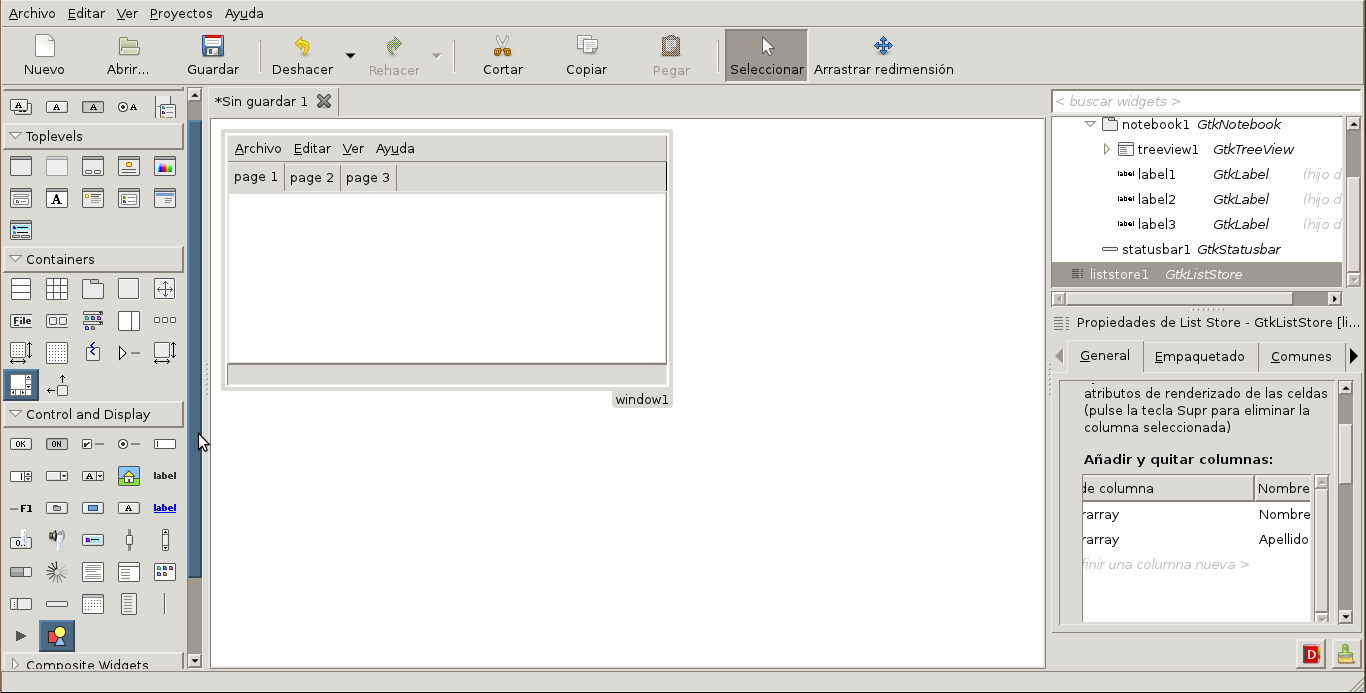
\includegraphics[height=5cm]{glade_shot.png}
    \end{center}
  \end{frame}
  
  \section{Algo de código}
  
  \begin{frame}[containsverbatim]
    \frametitle{Básico}
    \begin{verbatim}
import gtk

window = gtk.Window()
window.show()

gtk.main()
    \end{verbatim}
  \end{frame}
  
  \begin{frame}[containsverbatim]
    \frametitle{Insertando algun widget}
    \begin{verbatim}
...
button = gtk.Button()
button.show()
window.add(button)
...
    \end{verbatim}
  
  \end{frame}
  
  \begin{frame}[containsverbatim]
    \frametitle{Cambiando información de un widget.}
    \begin{verbatim}
...
button.set_label("Pulse Aquí")
...
    \end{verbatim}
  \end{frame}
  
  \begin{frame}[containsverbatim]
    \frametitle{Conectando una señal}
    \begin{verbatim}
...
button.connect("clicked",boton_clickeado)
...
    \end{verbatim}
  \end{frame}

  \begin{frame}[containsverbatim]
    \frametitle{Definiendo un manejador}
    \begin{verbatim}
...
def boton_clickeado(widget):
	print "hola mundo"
...
    \end{verbatim}
  \end{frame}

  \begin{frame}[containsverbatim]
    \frametitle{Importar un interfaz generado}
    \begin{verbatim}
...
builder = gtk.Builder()
builder.add_from_file("ruta/archivo.glade")
...
    \end{verbatim}
  \end{frame}

  \begin{frame}[containsverbatim]
    \frametitle{Conectar las señales}
    \begin{verbatim}
...
builder.connect_signals(locals())
...
    \end{verbatim}
  \end{frame}

  \section{Ejemplos}

  \begin{frame}[containsverbatim]
    \frametitle{Chrome en 30 lineas}
    Ejemplo de insertar un webkit en una aplicación GTK
  \end{frame}

  \begin{frame}[containsverbatim]
    \frametitle{Sumadora}
    Ejemplo de una sumadora que utiliza un XML de glade para generar el interfaz.
  \end{frame}
  
  \section*{Para terminar}
 
  \begin{frame}
    \frametitle{Referencias}
    \begin{itemize}
      \item ¿Por dónde empezar?
        \begin{itemize}
	  \item \url{http://www.pygtk.org}: Referencia completa.
        \end{itemize}
      \item ¿Dónde preguntar?
        \begin{itemize}
	  \item Lista de correo de python-es: python-es@python.org
	  \item Listas de distribución de grupos de usuarios de Linux: gul@gul.uc3m.es
        \end{itemize}
    \end{itemize}
  \end{frame}

  \begin{frame}
    \frametitle{Dudas}
    \dots
  \end{frame}
  
  \begin{frame}
    \frametitle{\begin{center}Fin\end{center}}
  \end{frame}

\end{document}
